%!TEX root = tapp_whatif.tex
\section{Introduction}
\label{sec:introduction}
What-if analysis~\cite{hung17,deutch13} determines how a hypothetical update to a database instance affects the result of a query.
Consider the following what-if query: \textit{``How would a 10\% increase in sales  affect our company’s revenue this year?''}
While the result of this query can help an analyst to understand how revenue is affected by sales,
its practical utility is limited because it does not provide any insights about how this increase in sales could have been achieved in the first place.
We argue that this problem is not specific to this example, but rather is a fundamental issue with classical what-if analysis since the hypothetical update to the database is part of the input.
We propose \emph{historical what-if queries} (\emph{\abbrHW}), a novel type of what-if queries where the user postulates a hypothetical change to the transactional history of the database.





% which defines such changes based on past business operations and historical transactions so achieving such changes is clear and answering such queries can help users to decide about their future policies and business operations. . Since this change is based on the past update operation that was executed on the database in the past, it is easy for the user to implement this change again and he can decide whether to change their business operations or keep it like before.


% It gives an insight that how increasing sales can affect the revenue but answering "how sales can be increased?" is a harder question and ambiguous.

% The answer to a what-if query explains how the query's result would change if the update would have been applied to the database.

% postulates a hypothetical update to a database and explains
% can be used to
% determine how a query's result would change based on hypothetical changes to a database. It helps users to understand how a change to data could affect the result of a query. However, it is usually unclear how such a change could have been happened.

% To make this approach efficient we develop static (schema-level) and dynamic analysis techniques for transactional workloads that enable use omit replaying transactions if that are not affected by the hypothetical change to the history.

%Answering such \textit{what-if queries} amounts to efficiently maintaining view (the query result) under updates.


%What-if queries are often realized using incremental view maintenance (e.g.,~\cite{deutch13,hung17,ZG95}) to avoid having to fully reevaluate the query over the input incorporating the hypothetical changes.
% to determine the effect the change has on the query's output.
%An example for a What-if query is: \textit{``How would a 10\% increase in sales % in California
%  affect my company’s revenue this year?''}
%While a what-if query provides insight into how a change to data would affect the result of a query, % it is often hard for a user to formulate such hypothetical changes to the database,
% % because
%it does not answer the important question of how such a change % of the database state
%could have been achieved. For instance, how to increase % the
%sales % in California
%by 10\% is potentially a much harder question to answer than determining the effect of this  increase % in sales
%on % the company's
%revenue.
%  Such changes are typically based on past operations.
% In fact, it may be much easier for the user to formulate what-if questions as changes to past actions (the history of the database) instead of changes to the current database state. For example: \textit{``How would revenue be affected if we would have charged 5\% interest for account overdrafts instead of 10\%?''}  Such a question can be interpreted as hypothetical changes to update operations or database transactions executed in the past, e.g., changing all past updates that applied interest to a user's account to use an interest rate of \%5. Importantly, the answer to such a question is more likely to lead to actionable insights.
% If the  hypothetical change to overdraft interest would result in a significant increase in revenue, then it is immediately clear how to implement this change --- by decreasing the overdraft interest. % While this example may be a bit contrived,
% This example illustrates the fundamental difference between regular what-if queries that propose a change to the data and \emph{historical what-if queries}, the new type of predictive queries that we propose in this work, which postulate a change to past database operations.
%We refer such queries that ask questions about hypothetical changes to a transactional history as \emph{historical what-if} queries.
%  In this work we study how to efficiently answer such queries, i.e., how to effectively determine the changes to the current database state (or to a view over the current database) based on hypothetical changes to the database history. We exploit a declarative replay technique called reenactment we have developed in previous work that replays a transactional workload or part thereof using temporal queries. Reenactment enables us to replay hypothetical histories to determine their effect on the current data or the  result of an analysis query.
% To make this approach efficient we develop static (schema-level) and dynamic analysis techniques for transactional workloads that enable use omit replaying transactions if that are not affected by the hypothetical change to the history.

%%%%%%%%%%%%%%%%%%%%%%%%%%%%%%%%%%%%%%%%
\begin{figure}[t]
  \centering

    \resizebox{1\columnwidth}{!}{
      \begin{minipage}{1.5\columnwidth}
        \centering
        {\bf\large Order}\\[1mm]
    \begin{tabular}{|c|c|c|c|c|l}
      \thead{ID} & \thead{Customer} & \thead{Country} & \thead{Price} & \thead{ShippingFee} & \\ \cline{1-5}
       % $\cMarker{T_0}{6}{1}(\upMarker{I}{T_0}{2}{1}(x_1))$ &
                                                          11 & Susan  & UK &  20 &  5 & $o_1$ \\
    % $\cMarker{T_0}{6}{2}(\upMarker{I}{T_0}{3}{2}(x_2))$ &
      12 & Alex  & UK &  50 & 5 & $o_2$ \\
    % $\cMarker{T_0}{6}{4}(\upMarker{I}{T_0}{4}{3}(x_3))$ &
                                                          13 & Jack  & US &  60 & 3 & $o_3$ \\
       % $\cMarker{T_0}{6}{4}(\upMarker{I}{T_0}{5}{4}(x_4))$ &
                                                          14 & Mark  & US &  30 & 4 & $o_4$ \\ \cline{1-5}
    \end{tabular}
  \end{minipage}
} \vspace{-3mm}
  \caption{Running example database instance.}
  \label{fig:running-example-instance}
  \vspace{-4mm}
\end{figure}
%%%%%%%%%%%%%%%%%%%%%%%%%%%%%%%%%%%%%%%%
\begin{figure}[t]
  % \centering
  \resizebox{1\columnwidth}{!}{
    \begin{minipage}{1.5\linewidth}
      \centering
      \begin{tabular}{|l|l|c|}
        \hline
        \thead{U}                          & \multicolumn{1}{c|}{\thead{SQL}}                                                              \\ \hline
        \rowcolor{shadeblue}     $u_1$     & \lstinline! UPDATE Order SET ShippingFee=0  WHERE Price>=50;!                                \\  [1mm]
        \rowcolor{pink}         ${u_1}'$   & \lstinline! UPDATE Order SET ShippingFee=0  WHERE Price>=60;!                                \\ [1mm]
        $u_2$                              & \lstinline!  UPDATE Order SET ShippingFee=ShippingFee+5 WHERE Country='UK' AND Price <=100;!  \\[1mm]
        \rowcolor{shadeblue}        $u_3$  & \lstinline! UPDATE Order SET ShippingFee=ShippingFee-2 WHERE Price <=30 AND ShippingFee>=10;! \\ [1mm]
        \hline
      \end{tabular}
    \end{minipage}
  }                                                                                                                                       \\[-3mm]
  \caption{History $\history$ implementing the shipping fee policy and a hypothetical change of the policy (update ${u_1}'$ replaces $u_1$ to raise the price for waiving shipping fees to \$60).}
  \label{fig:Transitive-Transactions-Example}
\end{figure}
%%%%%%%%%%%%%%%%%%%%%%%%%%%%%%%%%%%%%%%%
%%%%%%%%%%%%%%%%%%%%%%%%%%%%%%%%%%%%%%%%
% \begin{figure}[t]
%   $,$                                                                                                                                                  \\[-7mm]
%   \centering
%   \resizebox{1\columnwidth}{!}{
%   \begin{minipage}{1.5\columnwidth}
%     \centering {\large \bf Order}                                                                                                                     \\[2mm]
%     \begin{tabular}{|c|c|c|c|c|c|c|l}
        %         \thead{ID} & \thead{Customer} & \thead{Item} & \thead{Quantity} & \thead{Price} & \thead{ShippingFee} & \thead{Status} &                       \\ \cline{1-7}
        %       %         $\cMarker{T_0}{6}{1}(\upMarker{I}{T_0}{2}{1}(x_1))$ &
                                                                                %                                                                                 11 & Susan  & X &  1 & 20 & 5 & Shipped & $o_1$                                            \\
                                                                                %    %                                                                                 $\cMarker{T_0}{6}{2}(\upMarker{I}{T_0}{3}{2}(x_2))$ &
                                                                                                                                                                                                                             %                                                                                                                                                                                                                              12 & Alex  & X &  2 & 20 & 5 & Received & $o_2$                                                                                                \\
                                                                                                                                                                                                                             %    %                                                                                                                                                                                                                              $\cMarker{T_0}{6}{4}(\upMarker{I}{T_0}{4}{3}(x_3))$ &
                                                                                                                                                                                                                                                                                                                                                                                                                                                                                                                       %                                                                                                                                                                                                                                                                                                                                                                                                                                                                                                                        13 & Jack  & Y &  2 & 30 & 3 & Received & $o_3$                                            \\
                                                                                                                                                                                                                                                                                                                                                                                                                                                                                                                       %       %                                                                                                                                                                                                                                                                                                                                                                                                                                                                                                                        $\cMarker{T_0}{6}{4}(\upMarker{I}{T_0}{5}{4}(x_4))$ &
                                                                                                                                                                                                                                                                                                                                                                                                                                                                                                                                                                                                                                                                                                                                                                                                                                                                                                                                                                                                                                                                                                              %                                                                                                                                                                                                                                                                                                                                                                                                                                                                                                                                                                                                                                                                                                                                                                                                                                                                                                                                                                                                                                                                                                               14 & Mark  & Z &  6 & 10 & 4 & Canceled & $o_4$                                            \\ \cline{1-7}
        %       \end{tabular}
        %         \end{minipage}
        %         }                                                                                                                                                    \\[-3mm]
        %         \caption{Database state after executing the original history}
        %         \label{fig:updated-example-instance}
        %%       \end{minipage}
        %         \end{figure}
        % %%%%%%%%%%%%%%%%%%%%%%%%%%%%%%%%%%%%%%%%
        %%%%%%%%%%%%%%%%%%%%%%%%%%%%%%%%%%%%%%%%
\begin{figure}[t]
  $\,$                                                                                                                                                   \\[-5mm]
  \centering
  \begin{minipage}{1\linewidth}
    \centering
    \resizebox{1\columnwidth}{!}{
      \begin{minipage}{1.5\columnwidth}
        \centering {\large \bf Order}                                                                                                                      \\[2mm]
        \begin{tabular}{|c|c|c|c|c|l}
          \thead{ID}                                                                                                                                                                                                                         & \thead{Customer} & \thead{Country} & \thead{Price} & \thead{ShippingFee} & \\ \cline{1-5}
          % $\cMarker{T_0}{6}{1}(\upMarker{I}{T_0}{2}{1}(x_1))$                                                                                                                                                                              &
                                                                  11                                                                                                                                                                         & Susan            & UK              & 20            & 8                   & $o_5$                                                        \\
                                                                  % $\cMarker{T_0}{6}{2}(\upMarker{I}{T_0}{3}{2}(x_2))$                                                                                                                      &
                                                                                                                          12                                                                                                                 & Alex             & UK              & 50            & 5                   & $o_6$ \\
                                                                                                                          % $\cMarker{T_0}{6}{4}(\upMarker{I}{T_0}{4}{3}(x_3))$                                                              &
                                                                                                                                                                                  13                                                         & Jack             & US              & 60            & 0                   & $o_7$                                                          \\
                                                                                                                                                                                  % $\cMarker{T_0}{6}{4}(\upMarker{I}{T_0}{5}{4}(x_4))$      &
                                                                                                                                                                                                                                          14 & Mark             & US              & 30            & 4                   & $o_8$                                                           \\ \cline{1-5}
        \end{tabular}
      \end{minipage}
    }                                                                                                                                                     \\[-3mm]
    \caption{Result of  executing the original history $\history$.}
    \label{fig:updated-example-instance}
  \end{minipage}
  % \begin{minipage}{0.27\linewidth}
  %   \centering
  %   \resizebox{1\columnwidth}{!}{
  %   \begin{minipage}{1.5\columnwidth}
  %     \centering {\large \bf Query result}                                                                                                                \\[2mm]
  %     \begin{tabular}{|c|c|l}
  %       \thead{Total} & \thead{Country}&                                                                                                                \\ \cline{1-2}
  %       73 & UK & $o'_1 + o''_2$                                                                                                                         \\
  %       94 & US & $o'_3 + o_4$                                                                                                                           \\
  %       \cline{1-2}
  %     \end{tabular}
  %   \end{minipage}
  % }                                                                                                                                                     \\[-3mm]
  %   \caption{$\query_{total}$ result}
  %   \label{fig:original-query-result}
  % \end{minipage}
\end{figure}
% %%%%%%%%%%%%%%%%%%%%%%%%%%%%%%%%%%%%%%%%
% %%%%%%%%%%%%%%%%%%%%%%%%%%%%%%%%%%%%%%%%
\begin{figure}[t]
  $\,$                                                                                                                                                   \\[-5mm]
  \centering
  \begin{minipage}{1\linewidth}
    \centering
    \resizebox{1\columnwidth}{!}{
      \begin{minipage}{1.5\columnwidth}
        \centering {\large \bf Order}                                                                                                                      \\[2mm]
        \begin{tabular}{|c|c|c|c|c|l}
          \thead{ID}                                                                                                                                                                                                                         & \thead{Customer} & \thead{Country} & \thead{Price} & \thead{ShippingFee}    & \\ \cline{1-5}
          % $\cMarker{T_0}{6}{1}(\upMarker{I}{T_0}{2}{1}(x_1))$                                                                                                                                                                              &
                                                                  11                                                                                                                                                                         & Susan            & UK              & 20            & 8                      & $o_5$ \\
                                                                  % $\cMarker{T_0}{6}{2}(\upMarker{I}{T_0}{3}{2}(x_2))$                                                                                                                      &
                                                                                                                          12                                                                                                                 & Alex             & UK              & 50            & \cellcolor{shadered}10 & $o_6'$ \\
                                                                                                                          % $\cMarker{T_0}{6}{4}(\upMarker{I}{T_0}{4}{3}(x_3))$                                                              &
                                                                                                                                                                                  13                                                         & Jack             & US              & 60            & 0                      & $o_7$                                                          \\
                                                                                                                                                                                  % $\cMarker{T_0}{6}{4}(\upMarker{I}{T_0}{5}{4}(x_4))$      &
                                                                                                                                                                                                                                          14 & Mark             & US              & 30            & 4                      & $o_8$                                                           \\ \cline{1-5}
        \end{tabular}
      \end{minipage}
    }                                                                                                                                                     \\[-3mm]
    \caption{Result of executing the hypothetical history $\ahmod$.}
    \label{fig:whatif-example-instance}
  \end{minipage}
  % \begin{minipage}{0.27\linewidth}
  %   \centering
  %   \resizebox{1\columnwidth}{!}{
  %     \begin{minipage}{1.5\columnwidth}
  %       \centering {\large \bf Query result}                                                                                                                \\[2mm]
  %       \begin{tabular}{|c|c|l}
  %         \thead{Total} & \thead{Country}                                                                                                                 \\ \cline{1-2}
  %         \cellcolor{shadered}78 & UK & $o'_1 + o'_2$                                                                                                     \\
  %         94 & US & $o'_3 + o_4$                                                                                                                           \\
  %         \cline{1-2}
  %       \end{tabular}
  %     \end{minipage}
  %   }                                                                                                                                                     \\[-3mm]
  %   \caption{$\query_{total}$ result}
  %   \label{fig:whatif-query-result}
  % \end{minipage}
\end{figure}
%%%%%%%%%%%%%%%%%%%%%%%%%%%%%%%%%%%%%%%%.

% %%%%%%%%%%%%%%%%%%%%%%%%%%%%%%%%%%%%%%%%
% \begin{figure*}[t]
%   \centering
%   \begin{minipage}{0.49\linewidth}
%   \centering
%     \resizebox{1\columnwidth}{!}{
%   \begin{minipage}{1.4\columnwidth}
%    \centering {\large \bf Employee}\\[2mm]
%     \begin{tabular}{l|c|c|c|c|c|l}
%      & \thead{ID} & \thead{Name} & \thead{Calls} & \thead{Sales} & \thead{Bonus} & \\ \cline{2-6}
%     $\cMarker{T_1}{22}{1}(\upMarker{U}{T_1}{21}{1}(\cMarker{T_0}{6}{1}(\upMarker{I}{T_0}{2}{1}(x_1)))$ & 101 & David Spears & 18 &  15 & 0 & $e'_1$ \\
% $\cMarker{T_0}{6}{2}(\upMarker{I}{T_0}{3}{2}(x_2))$ & 102 & Mark Smith & 40 &  20 & 100 & $e_2$ \\
%     $\cMarker{T_0}{6}{3}(\upMarker{I}{T_0}{4}{3}(x_3))$ &  103 & Susan Sommers & 80 &  50 & 200 & $e_3$ \\
%      $\cMarker{T_2}{24}{4}(\upMarker{U}{T_2}{23}{4}(\cMarker{T_0}{6}{4}(\upMarker{I}{T_0}{5}{4}(x_4)))$ &  104 & Robert Singer & 120 &  80 & 350 & $e'_4$ \\ \cline{2-6}
%     \end{tabular}
%   \end{minipage}
% }
%   \caption{Database state after executing the original history}
%   \label{fig:updated-example-instance}
% \end{minipage}
% % \end{figure}
% % %%%%%%%%%%%%%%%%%%%%%%%%%%%%%%%%%%%%%%%%
% % %%%%%%%%%%%%%%%%%%%%%%%%%%%%%%%%%%%%%%%%
% % \begin{figure}[t]
%   \begin{minipage}{0.49\linewidth}
%   \centering
% \resizebox{1\columnwidth}{!}{
%   \begin{minipage}{1.4\columnwidth}
%    \centering {\large \bf Employee}\\[2mm]
%     \begin{tabular}{l|c|c|c|c|c|l}
%       & \thead{ID} & \thead{Name} & \thead{Calls} & \thead{Sales} & \thead{Bonus} & \\ \cline{2-6}
%     $\cMarker{T_1}{22}{1}(\upMarker{U}{T_1}{21}{1}(\cMarker{T_0}{6}{1}(\upMarker{I}{T_0}{2}{1}(x_1)))$ & 101 & David Spears & 18 &  15 & 0 & $e'_1$ \\
% $\cMarker{T_3}{26}{2}(\upMarker{U}{T_3}{25}{2}(\cMarker{T_1}{22}{2}(\upMarker{U}{T_1}{21}{2}(\cMarker{T_0}{6}{2}(...)))$ & 102 & Mark Smith & 40 &  20 & \cellcolor{shadered} 150 & $e"_2$ \\
%     $\cMarker{T_0}{6}{3}(\upMarker{I}{T_0}{4}{3}(x_3))$ &  103 & Susan Sommers & 80 &  50 & 200 & $e_3$ \\
%      $\cMarker{T_2}{24}{4}(\upMarker{U}{T_2}{23}{4}(\cMarker{T_0}{6}{4}(\upMarker{I}{T_0}{5}{4}(x_4)))$ &  104 & Robert Singer & 120 &  80 & 350 & $e'_4$ \\ \cline{2-6}
%     \end{tabular}
%   \end{minipage}
% }
%   \caption{Database state based on the historical what-if query}
%   \label{fig:whatif-example-instance}
% \end{minipage}

% \end{figure*}
% %%%%%%%%%%%%%%%%%%%%%%%%%%%%%%%%%%%%%%%%.

%%%%%%%%%%%%%%%%%%%%%%%%%%%%%%%%%%%%%%%%
\begin{exam}
  \label{ex:running-example}

  Consider an online retailer that has developed a new shipping fees policy. An example database instance is shown in \Cref{fig:running-example-instance}.
\iftechreport{
  The new policy was implemented by updating the shipping fees for existing orders as follows: %\emph{Bonus} based on the number of sales \emph{Calls}:
the fee for orders with price equal or greater than \$50 was set to \$0, orders of less than or equal to \$100 with a destination in the UK were charged an additional \$5 shipping fee, and orders with a  price equal or less than \$30 and shipping fee equal or more than \$10 received a \$2 discount for their shipping fee.} \Cref{fig:Transitive-Transactions-Example} shows a transactional history with three updates $\up_1$, $\up_2$ and $\up_3$ that implement this policy which % were executed sequentially in the  order shown here
% resulting
resulted in the database state shown in \Cref{fig:updated-example-instance}. % Ignore update $u_1'$ shown with red background for now.
For example, $\up_1$ waives shipping fees for orders of at least \$50.
Bob, an analyst, wants to understand how a larger order price threshold for waiving shipping fees, say \$60, would have affected revenue.
% This question corresponds to the historical what-if query: \textit{``How would revenue be affected if we would have used  a threshold of \$60 instead of \$50 for waiving  shipping fees?''}. This query changes the history by replacing the \lstinline!WHERE! clause of update $u_1$ to \lstinline!WHERE Price >= 60! (update ${\up_1}'$ shown in \Cref{fig:Transitive-Transactions-Example}).
Bob's request can be expressed as a \emph{historical what-if query} which replaces the update $\up_1$ with update ${\up_1}'$ (highlighted in red in \Cref{fig:Transitive-Transactions-Example}). \Cref{fig:whatif-example-instance} shows the new state of the database after executing the modified transactional history over the database from \Cref{fig:running-example-instance}. % \Cref{fig:original-query-result} shows the original and result of $\query_{total}$.
% The result of this query over the database produced by the hypothetical history is shown in \Cref{fig:whatif-query-result}.
The hypothetical change results in an increase of the shipping fee for the record with ID 12 (highlighted in red).
By evaluating the effect of changing a past action (an update) instead of changing the current state of the database as in classical what-if analysis,
the answer to a historical what-if query can inform future actions. For example, if revenue is increased significantly by using a \$60 cutoff for waiving shipping fees, then we may apply this higher threshold in the future.
%   This policy was implemented though the update shown below (the database schema is shown in \Cref{fig:running-example-instance}):
% %
% \begin{lstlisting}
% UPDATE Order SET ShippingFee=0 WHERE Price>=50;
% \end{lstlisting}
% %
%In this example, we examine the transitive dependency of transactions.
%Consider the order table for an online retailer shown in \Cref{fig:running-example-instance}. % (ignore annotations for now)
% stores order information like \emph{ID}, \emph{Price}, and \emph{Shipping Fee} and customer information such as \emph{Customer} (customer name), and \emph{Country} (country of residency).
%
%The retailer did introduce
% as shown in \Cref{fig:Transitive-Transactions-Example}. The result of the this history is shown in \Cref{fig:updated-example-instance}.
% \footnote{As we will discuss further in \Cref{sec:approach}, our approach also handles concurrent execution of transactions - even under lower isolation levels}
%Bob, a manager at the retailer, requests a report on how raising the minimum order price from \$50 to \$60  for reducing the shipping fee (update $\up_1$) would impact  revenue
% The revenue per country can be computed using a query $\query_{total}$:
% \begin{lstlisting}
% SELECT sum(Price+ShippingFee) AS Total, Country
% FROM Order
% GROUP BY Country
% \end{lstlisting}
% Bob's request can be expressed as a \emph{historical what-if query} which replace the update $u_1$ with update ${u_1}'$ that is highlighted in red in \Cref{fig:Transitive-Transactions-Example}. \Cref{fig:whatif-example-instance} shows the new state of the order database after executing the modified transactional history over the database from \Cref{fig:running-example-instance}. % \Cref{fig:original-query-result} shows the original and result of $\query_{total}$.
% % The result of this query over the database produced by the hypothetical history is shown in \Cref{fig:whatif-query-result}.
% Note that the hypothetical change results in an increase in the shipping fee for the record with ID 12 (highlighted in red).
\end{exam}
%%%%%%%%%%%%%%%%%%%%%%%%%%%%%%%%%%%%%%%%

In this paper, we study how to efficiently answer
historical what-if queries (\abbrHWs) such as the one from \Cref{ex:running-example}.
A \abbrHW $\hwhatif$ is a triple $(\history, \db, \deltaHist)$ where $\history$ is a transactional history (a sequence of insert/update/delete statements), $\db$ is the state of the database before the execution of the transactional history $\history$, and $\deltaHist$ is a set of modifications to the history, i.e., it replaces some updates from $\history$ with hypothetical updates (or inserts new / deletes existing update statements). We use $\ahmod$ to denote the history that is the result of applying $\deltaHist$ to $\history$. The result of $\hwhatif$ is the symmetric difference ($\Delta$) of the database instances produced by evaluating $\history$ ($\history[\deltaHist$]) over database $\db$, i.e., the set of tuples in the result of the history that are affected by the modification. For our running example, the symmetric difference  would contain the two versions of the tuple with ID 12 produced by the original and modified history. We focus on deterministic updates (given the same input, multiple executions of an update are guaranteed to return the same result).
%
The existence of an update in a transactional history is often dependent on the existence of other updates in the history and/or on external events (e.g., user interactions) which are not observed by the DBMS. For instance, if we delete a statement that inserted a customer, then this customer could have never submitted any orders. Consequently, all insert statements corresponding to orders by this customer should be removed. While dealing with such causal relationships is important for helping users to formulate realistic hypothetical scenarios, it is orthogonal to the problem we study in this work: how to efficiently answer \abbrHWs. Learning such causal relationships between the updates of a history % from past histories and/or background knowledge
  and then using them to augment a user-provided \abbrHW is an interesting and challenging problem that we leave to future work.
% and present an % initial
%approach for evaluating such queries over a database backend.

%%%%%%%%%%%%%%%%%%%%%%%%%%%%%%%%%%%%%%%%
\begin{figure}[t]
  \begin{minipage}{1.0\linewidth}
    \centering
    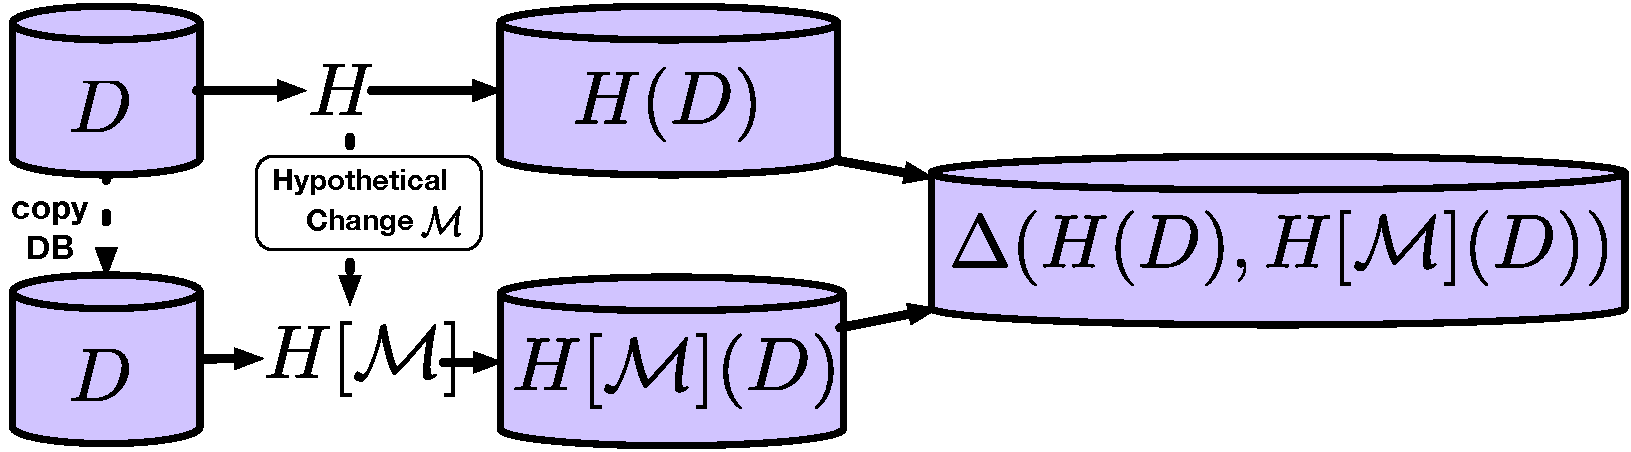
\includegraphics[width=0.9\linewidth]{brute-force-overview.pdf}
    \vspace{-4.5mm}
    \caption{The naïve method requires evaluating the modified history over a copy of the original database.}
    \label{fig:Naive-Method}
  \end{minipage}
  \begin{minipage}{1.0\linewidth}
    \centering
    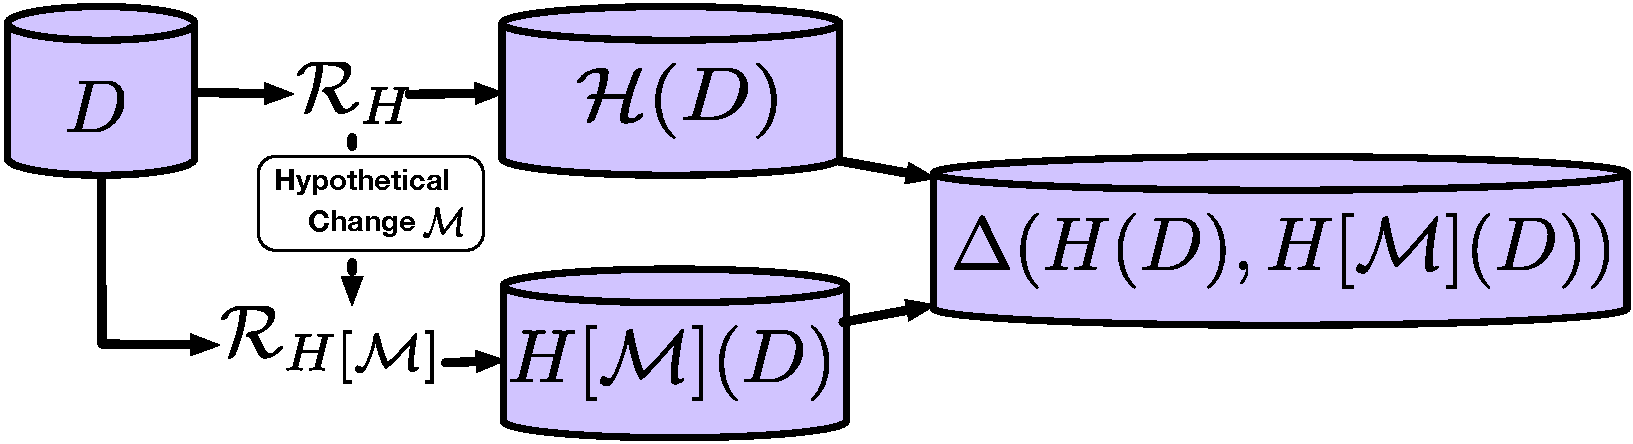
\includegraphics[width=0.9\linewidth]{reenact-overview.pdf}
    \vspace{-4.5mm}
    \caption{Reenactment-based method implemented in Mahif}
    \label{fig:Prop-Method}
  \end{minipage}
\end{figure}
%%%%%%%%%%%%%%%%%%%%%%%%%%%%%%%%%%%%%%%%

%%%%%%%%%%%%%%%%%%%%%%%%%%%%%%%%%%%%%%%%%%%%%%%%%%%%%%%%%%%%%%%%%%%%%%%%%%%%%%%%
A \textbf{naïve approach} for answering a \abbrHW is shown in \Cref{fig:Naive-Method}. This method creates a copy of the database as it was before the execution of the first update that has been modified by $\deltaHist$, and then executes the modified history on this copy. % It then executes the requested query on the copied database and the original. Finally, i
It then computes the symmetric difference between the current database state (which is the result of evaluating the original transactional history $\history$ over $\db$) and the database state that is the result of evaluating the modified history $\ahmod$ over the copy of database $\db$.  % is the answer to the historical what-if query. Note that
Note that this requires access to a past database state $\db$ before the execution of the first update of the history, e.g., we can use a DBMS with support for \textit{time travel} to access $\db$ (e.g., Oracle, SQLsever, DB2).
% The disadvantages of the naive method are non-trivial.
The naïve method requires additional storage to store the copy of $\db$ and the evaluation of the modified history results in a large amount of write I/O. % for updating data and write-ahead logging (WAL).
% Creating a copy of the database and evaluating the modified history results in a large amount of write I/O.
%Moreover, most database systems log modifications of update operations using write-ahead logging (WAL) for recovery purposes, whose cost is prohibitive for evaluating or replaying a large number of updates.
% While some systems allow WAL to be deactivated,
        %         for temporary tables,
However, an even larger concern is that the modifications  $\deltaHist$ may only affect a small fraction of the data and many updates in the history may be irrelevant for computing the symmetric difference. % That is, evaluating all updates of the modified history over all tuples in $\db$ is likely to be overkill.


%(no matter whether real or hypothetical) using temporal queries.
% Such queries can be executed using any DBMS with support for \textit{time travel} (e.g., Oracle, DB2, SQLsever).
% \BGDel{Time travel can be implemented using triggers for systems that do not support this functionality natively.}{too detailed for intro}
        %         The naive solution to implement historical what-if queries is to reevaluate the modified history to produce an updated database state. Afterwards, we evaluate the user provided query over both the current database state and the updated database state and then determine what has changed.

%%%%%%%%%%%%%%%%%%%%%%%%%%%%%%%%%%%%%%%%%%%%%%%%%%%%%%%%%%%%%%%%%%%%%%%%%%%%%%%%
Our \textbf{proposed method} is shown in \Cref{fig:Prop-Method}. In order to overcome the limitations of the naïve method, we propose Mahif as a system that answers \abbrHWs using reenactment~\cite{AG14,AG17,AG18}%  which is a declarative replay technique for transactional history by a temporal query.
% Our approach is based on reenactment~\cite{AG14,AG17}, %a technique we have developed
, a declarative technique for replaying transactional histories using queries.
% Like the naïve method,
Our approach also uses time travel to access $\db$, the state of the database just before the time the first modified update was executed. In contrast to the naïve method, the database does not need to be copied. % Instead, time travel is used to get the state of the database before the update that is being modified, which is then the beginning state of the reenactment.
Instead, the modified history is reenacted over $\db$ by running a query $\ract{\ahmod}$.
Thus, reenactment has the advantage of not incurring write I/O.
The result of query $\ract{\ahmod}$ is equal to the result of executing $\ahmod$ over $\db$.  % to the naive method, we run the requested query on the result of the reenactment and original database state and then
We then compute the symmetric difference between the result of the modified history (returned by $\ract{\ahmod}$) and the current database state ($\history(\db)$) computed by reenacting $\history$ over $\db$. Reenacting $\history$, while seemingly redundant, allows us to develop novel optimizations which % dramatically decrease the amount data that needs to be processed and enables us to
exclude irrelevant updates from the history and irrelevant data from reenactment. % if they provably have no effect on the answer of the historical what-if query.
 % and, by evaluating a history as a single query enables the DBMS to optimize across statements in the history.

% The main advantage of using reenactment lies in these optimization, but reenactment has the additional advantage that it does not incur write I/O and that many small operations (the update statement of the history) are replaced with a single query enabling the database's query optimizer to optimize across multiple statements in the history. % as well as enabling the aforementioned optimizations.

% One advantage of using reenactment is it does not need to copy the database. Reenactment avoids the logging overhead caused by running updates. Also, it enables optimizations such as program slicing that minimize the number of updates to reenact and data slicing which reduces input data into the reenactment.
%%%%%%%%%%%%%%%%%%%%%%%%%%%%%%%%%%%%%%%%%%%%%%%%%%%%%%%%%%%%%%%%%%%%%%%%%%%%%%%%
\partitle{Program Slicing}
To be able to identify updates that can safely be excluded from the evaluation of an \abbrHW, we introduce the notion of a \emph{slice}. A slice for a \abbrHW $\hwhatif$ is a subset of the updates from $\history$ and $\ahmod$ that is sufficient for computing the result of $\hwhatif$. We identify a property called tuple-independence which holds for a large class of updates (corresponding to SQL update and delete statements without joins and subqueries, and \lstinline!INSERT ... VALUES ...! statements). Tuple independence ensures that we can determine whether a subset of updates is a slice by testing for each individual tuple from the database whether the subset produces the same result for $\hwhatif$ than for the full histories. To improve the efficiency of slicing, we compress $\db$ into a set of constraints that compactly over-approximate the database. Inspired by program slicing and symbolic execution techniques~\cite{bucur14,luckow14}, and ideas from incomplete databases~\cite{AG85,IL84a}, we develop a technique that evaluates updates from a history over a single tuple symbolic instance (a tuple with variables as attribute values) subject to the constraints from the compressed database. The result of symbolic evaluation is a single tuple symbolic instance that encodes all possible tuples in the result of the history for any input tuple fulfilling the compressed database constraints. We then use a constraint solver % (MILP solver in our case)
  to determine whether a candidate slice produces the same result for $\hwhatif$ as the full histories for every possible input tuple. If that is the case, then it is safe to use the slice instead of $\history$ and $\ahmod$ to answer $\hwhatif$.
The cost of program slicing only depends on the number of updates in the history and the size of the constraints encoding the data distribution of the database. %Thus, % this method
% is suited well for larger database instances and
% allows us to
%         we can trade performance of program slicing for reduced slice size by tuning the compression.


% Towards this goal we propose a \textit{program slicing method} that  statically analyzes potential
% %provenance
% dependencies among updates in a history and excludes updates from reenactment if we can prove that their exclusion will not affect the result of the historical what-if query. Technically, our method
% is inspired by program slicing and symbolic execution techniques from the programming languages community~\cite{bucur14,luckow14}.
% % This method is similar to ideas from programming languages, i.e., symbolic execution~\cite{bucur14,luckow14}.
% % and constraint databases \cite{gomez14,kuper13}.
% We simulate updates in the history through symbolic execution to determine updates that may dependent on updates modified by a historical what-if query. We formalize symbolic execution using ideas from incomplete databases~\cite{AG85,IL84a}.
% Dependent updates may produce different  outputs in the original and modified history. In order to improve performance of our approach, we just consider dependent updates in reenactment as only these updates may  affect the final result of the historical what-if query.

%%%%%%%%%%%%%%%%%%%%%%%%%%%%%%%%%%%%%%%%%%%%%%%%%%%%%%%%%%%%%%%%%%%%%%%%%%%%%%%%
\partitle{Data Slicing}
We also propose \emph{data slicing} to prune data that we can prove is irrelevant for computing the answer to a \abbrHW. Based on the observation that any tuple in the symmetric difference has to be affected by at least one statement that was modified by $\deltaHist$, we filter the input of reenactment to remove tuples which are guaranteed to not be affected by any update modified by $\deltaHist$. In addition to the class of queries supported by program slicing, data slicing is also applicable to insert statements with queries (\lstinline!INSERT ... SELECT! in SQL).
\BGDel{Our symbolic execution framework is of independent interest and can aide other static analysis task the require reasoning over multiple possible datasets or evaluation of updates over an incomplete database.}{Need space, maybe mention in future work}
%The proposed optimizations enables us exclude data from the replay (\textit{data slicing}) and to avoid replaying parts of the history (\textit{program slicing}).
%%%%%%%%%%%%%%%%%%%%%%%%%%%%%%%%%%%%%%%%
The main contributions of this paper are:
\begin{itemize}[noitemsep,topsep=0pt,parsep=0pt,partopsep=0pt,leftmargin=*]
%\item We formalize the problem of answering historical what-if queries.
% and provide related definitions to solve it.
%and detecting dependent updates.
\item
We formalize historical what-if queries and present a novel method for answering such queries based on reenactment.
%Our approach is based on \emph{reenactment}, a technique for replaying a transactional history using queries to avoid additional overhead of re-executing update in a transactional history and implement
% The reenactment query for a transaction $T$ is equivalent to $T$ within the context of a history under MV-semiring semantics, i.e., it returns the same database state % as the transaction
%  and has the same provenance. We reduce reenactment queries with MV-semiring semantics to queries in standard SQL that return a relational encoding of % of MV-semiring
%  provenance.

% \item We present our solution and algorithms for answering historical what-if queries.

\item We present two optimization techniques, \emph{program slicing} and \emph{data slicing}, which determine which updates and what data can be safely excluded when answering a \abbrHW.
  % hat determines statically whether updates from the history can be excluded from reenactment without affecting the results of the historical what-if query. For that we build a symbolic execution framework rooted in incomplete databases which allows us to encode the outcomes of a transactional history over all possible databases instances of a certain size. We then employ a constraint solver to compute a slice of the history, i.e., a subsequence  that is sufficient for answering the historical what-if query.

% \item We discuss an additional optimization technique---\emph{data slicing}---which filters the input data of a reenactment queries.

\item We demonstrate experimentally that our approach outperforms the naïve approach and that our optimizations result in significant additional performance improvements. % Note that the cost of program slicing is mostly determined by the number of updates in the history, but is independent of the database size. Thus, this method is suited well for larger database instances.

\end{itemize}

%%%%%%%%%%%%%%%%%%%%%%%%%%%%%%%%%%%%%%%%
% REMAINDER

% The remainder of the paper is organized as follows. We discuss background in \Cref{sec:background} and define historical what-if queries  in \Cref{sec:whif-def}. Afterwards, we discuss a naïve solution for our problem (\Cref{sec:naive-solution}) and then given an overview of our approach (\Cref{sec:overview}). \Cref{sec:filter} and \Cref{sec:dep-ana} introduces our data slicing and program slicing optimizations. In \Cref{sec:sym-exe} we introduce symbolic execution and explain how it is used for program slicing. % and how to translate and how a MILP solution is used to execute it(\Cref{sec:sym-lin}).
% In \Cref{sec:related-work}, we discuss related work, discuss experimental results in \Cref{sec:experiments}, and conclude in \Cref{sec:conclusions}.
%\BG{Remove SI ok?}
%%%%%%%%%%%%%%%%%%%%%%%%%%%%%%%%%%%%%%%%%
%\partitle{Snapshot Isolation} Snapshot isolation~\cite{BB95} is a widely applied multi-versioning concurrency control protocol. Under SI each trans\-ac\-tion $\xid$ sees a private snapshot of the database containing changes of transactions that have committed before $\xid$ started and $\xid$'s own changes. SI disallows concurrent transaction to update the same data item. This is typically implemented by using write locks where transactions waiting for a lock have to abort if the transaction currently holding the lock commits.
%%%%%%%%%%%%%%%%%%%%%%%%%%%%%%%%%%%%%%%%
%\subsection{Running Example}
%\label{sec:run-examp}
%We can consider different cases for a what-if query when we examine the effect of changing an update operation in a transaction on other transactions. For example, when a user wants to change an update operation in a transaction $T_1$, the other transaction $T_2$ that was executed after $T_1$ might be effected by this change or not. We state a transaction $T_2$ is depend on other transaction $T_1$  which includes what-if query if a tuple that is modified by the transaction $T_1$ was or would be also modified by the transaction $T_2$.
%%% Local Variables:
%%% mode: latex
%%% TeX-master: "historical_whatif"
%%% End:
